\documentclass[10pt]{article}

\usepackage[utf8]{inputenc}
\usepackage[american]{babel}
\usepackage{graphicx}
\usepackage{amsmath}
\usepackage{amsthm}
\usepackage{amssymb}
\usepackage{natbib}
\usepackage[margin=0.5in]{geometry}
\usepackage{fancyvrb}
\usepackage{Sweave}

\DefineVerbatimEnvironment{Sinput}{Verbatim}{xleftmargin=2em}
\DefineVerbatimEnvironment{Soutput}{Verbatim}{xleftmargin=2em}
\DefineVerbatimEnvironment{Scode}{Verbatim}{xleftmargin=2em}
\fvset{listparameters={\setlength{\topsep}{0pt}}}
\renewenvironment{Schunk}{\vspace{\topsep}}{\vspace{\topsep}}

\setlength{\parskip}{.1in}  
\setlength{\parindent}{0.0in}  

\setcounter{tocdepth}{1}
%\setcounter{secnumdepth}{1}

\newcommand{\R}{\textsf{R}}
\newcommand{\code}[1]{\texttt{#1}}
  
%\SweaveOpts{eps=FALSE, pdf=TRUE, png=TRUE, keep.source=FALSE, echo=TRUE, eval=TRUE}
  
\title{Potential distributions of \emph{Culex pipiens}, \emph{Culex quinquefasciatus}, and \emph{Culex salinarius} mosquitoes}
\author{John M. Drake}
  
\begin{document}
\Sconcordance{concordance:data-preparation.tex:data-preparation.Rnw:%
1 53 1 1 3 5 0 1 2 2 1 1 3 2 0 1 2 7 0 1 5 2 1 1 3 5 0 1 2 2 1 1 3 2 0 %
1 1 1 16 17 0 1 2 34 1 1 2 1 0 3 1 3 0 1 2 2 1 1 2 6 0 1 1 1 5 4 0 3 1 %
4 0 1 3 8 1 1 4 3 0 11 1 1 54 52 0 1 45 43 0 1 6 5 0 1 7 6 0 1 31 30 0 %
1 2 1 1 1 4 6 0 1 2 2 1 1 2 1 0 1 4 2 0 1 4 6 0 1 2 10 1 1 2 1 0 3 1 1 %
17 18 0 1 2 2 1 1 4 3 0 1 4 6 0 1 2 8 1 1 4 3 0 1 1 3 0 1 2 12 1 1 2 1 %
0 3 1 3 0 2 2 1 0 3 1 5 0 1 4 14 1 1 3 2 0 1 1 1 2 1 1 1 2 1 1 3 0 1 2 %
2 1 1 2 1 0 1 2 4 0 1 2 12 1 1 2 4 0 1 2 2 1 1 2 1 0 5 1 3 0 1 2 2 1 1 %
3 2 0 11 1 3 0 1 2 13 1 1 3 2 0 6 1 3 0 1 2 4 1 1 2 1 0 1 1 3 0 1 2 1 3 %
2 0 6 1 4 0 1 3 12 1 1 3 2 0 1 4 3 0 6 1 3 0 1 2 1 1}


\maketitle
  
\section{Introduction}
  
The goal of this study is to produce ecological niche models and maps of the potential distribution of three mosquitoes competent to transmit West Nile virus. This workflow derives from the earlier study of Drake \& Beier on the potential distribution of \textit{An. arabiensis} in Africa. Therefore, this initial work will focus on the potential distribution in Africa. Additional questions to be answered include:

\begin{enumerate}
  \item What is the right geographic scope of this study (Africa? Global?)
  \item If new data are acquired, should it be obtained at higher resolution?
  \item Should maps be projected in equal area format? (not relevant to data sampling, but possibly relevant to data thinning)
  \item Are projections for future climate desired?
  \item Are there relevant land use data that might be used as predictor variables?
\end{enumerate}

In addition, because of the aggregation of \textit{Culex} records, this study might provide a good opportunity to showcase the plug-and-play models. In this case, it may be desirable to compare thinned data (which are less susceptible to sampling heterogeneity, but fewer in number) and non-thinned data (which are expected to be more susceptible to sampling heterogeneity, here counteracted by the plug-and-play method). This study may be a good occasion to introduce the concept of ``data calibration''.


  
\begin{Schunk}
\begin{Sinput}
> #set up workspace
> rm(list=ls(all=TRUE))
\end{Sinput}
\end{Schunk}
  
Here we load the necessary libraries.
  
\begin{Schunk}
\begin{Sinput}
> #load libraries
> require(dismo)
> #require(raster)
> require(maptools)
> #require(spatstat)
> #require(rworldmap)
> #require(scatterplot3d)
\end{Sinput}
\end{Schunk}
  
Finally, we load some auxiliary functions
  
\begin{Schunk}
\begin{Sinput}
> #load auxiliary functions
> source('functions.R')   #project specific functions
\end{Sinput}
\end{Schunk}

Environmental data include baseline (average for years 1950-2000) and forecasted data for 2050 for Africa. Forecasted data were generated by the Hadley CM 3 model for scenario A1B, A2A, and B2A and have been statistically downscaled toa 10 minute resolution using the delta method. Raw data were obtained from \code{http://www.ccafs-climate.org/data/}. The environmental data are stored in R Data file \code{Africa.RData}. Scripts have been written to construct the environmental dataset from raw data files, but take a very long time to execute. Therefore, these data have been stored as an R workspace, which is loaded here.

\begin{Schunk}
\begin{Sinput}
> #load environmental data - baseline
> load('africa-baseline/Africa.RData')
> resolution <- res(environmental.data)
> #load environmental data - 2050 forecast (scenario A1B)
> #load('Africa-forecast-2050-A1B.RData')
> #data.a1b <- environmental.data.2050
> #rm(environmental.data.2050)
> 
> #load('Africa-forecast-2050-A2A.RData')
> #data.a2a <- environmental.data.2050
> #rm(environmental.data.2050)
> 
> #load('Africa-forecast-2050-B2A.RData')
> #data.b2a <- environmental.data.2050
> #rm(environmental.data.2050)
> 
> #load world map from maptools package
> data(wrld_simpl)
\end{Sinput}
\end{Schunk}

Environmental data include,

\begin{itemize}
\item Average monthly minimum temperature
\item Average monthly maximum temperature
\item Average monthly precipitation
\end{itemize}

as well as the 19 BIOCLIM variables

\begin{itemize}
\item (BIO1) Annual mean temperature
\item (BIO2) Mean diurnal range (Mean of monthly (max temp - min temp))
\item (BIO3) Isothermality (BIO2/BIO7) (* 100)
\item (BIO4) Temperature seasonality (standard deviation *100)
\item (BIO5) Maximum temperature of warmest month
\item (BIO6) Minimum temperature of coldest month
\item (BIO7) Temperature annual range (BIO5-BIO6)
\item (BIO8) Mean temperature of wettest quarter
\item (BIO9) Mean temperature of driest quarter
\item (BIO10) Mean temperature of warmest quarter
\item (BIO11) Mean temperature of coldest quarter
\item (BIO12) Annual precipitation
\item (BIO13) Precipitation of wettest month
\item (BIO14) Precipitation of driest month
\item (BIO15) Precipitation seasonality (coefficient of variation)
\item (BIO16) Precipitation of wettest quarter
\item (BIO17) Precipitation of driest quarter
\item (BIO18) Precipitation of warmest quarter
\item (BIO19) Precipitation of coldest quarter
\end{itemize}

Here we define some colors that will be useful for visualization.

\begin{Schunk}
\begin{Sinput}
> ose1 <- rgb(85,108,17, m=255)
> ose2 <- rgb(160,108,17, m=255)
> ose3 <- rgb(114,132,56, m=255)
> ose4 <- rgb(137,152,87, m=255)
\end{Sinput}
\end{Schunk}

We mask environmental data layers to points only on the African continent so that raster based computations (such as spatially averaged temperature or selection of random background points) may be performed.

\begin{Schunk}
\begin{Sinput}
> mask <- rasterize(wrld_simpl[wrld_simpl$REGION==2,], environmental.data)
\end{Sinput}
\begin{Soutput}
Found 57 region(s) and 135 polygon(s)
\end{Soutput}
\begin{Sinput}
> environmental.data <- mask(environmental.data, mask)
> #data.a1b <- mask(data.a1b, mask)
> #data.a2a <- mask(data.a2a, mask)
> #data.b2a <- mask(data.b2a, mask)
> #plot(environmental.data[[1]]/10)
> africa.lines <- wrld_simpl[(wrld_simpl$REGION==2 & wrld_simpl$NAME!='South Africa'),]
> SA <- wrld_simpl[(wrld_simpl$NAME=='South Africa'),]
> SA@polygons[[1]]@Polygons[[2]]@hole<-FALSE  # Here we take care of Lesotho
> africa.lines2 <- rbind(africa.lines, SA)
> #plot(africa.lines2, add=TRUE)
\end{Sinput}
\end{Schunk}

Now we construct some additional variables and normalize some variables. These include:
  
\begin{itemize}
\item Monthly temperature range (Monthly maximum temperature - Monthly minimum temperature)
\item log-transformations of strongly skewed variables
\item ecdf (percentile  of the empirical cumulative distribution function) transformations of extremely skewed variables
\end{itemize}

\begin{Schunk}
\begin{Sinput}
> #construct new variables and normalize data
> #x11(w=10,h=7); par(mfrow=c(3,4), mar=c(3,3,1,3))
> Jan.temp.diff<-environmental.data[[13]]-environmental.data[[1]];  #plot(Jan.temp.diff)  #January temperature range (in lieu of diurnal ranges)
> Feb.temp.diff<-environmental.data[[14]]-environmental.data[[2]];  #plot(Feb.temp.diff)  #February
> Mar.temp.diff<-environmental.data[[15]]-environmental.data[[3]];  #plot(Mar.temp.diff)  #March
> Apr.temp.diff<-environmental.data[[16]]-environmental.data[[4]];  #plot(Apr.temp.diff)  #April
> May.temp.diff<-environmental.data[[17]]-environmental.data[[5]];  #plot(May.temp.diff)  #May
> Jun.temp.diff<-environmental.data[[18]]-environmental.data[[6]];  #plot(Jun.temp.diff)  #June
> Jul.temp.diff<-environmental.data[[19]]-environmental.data[[7]];  #plot(Jul.temp.diff)  #July
> Aug.temp.diff<-environmental.data[[20]]-environmental.data[[8]];  #plot(Aug.temp.diff)  #August
> Sep.temp.diff<-environmental.data[[21]]-environmental.data[[9]];  #plot(Sep.temp.diff)  #September
> Oct.temp.diff<-environmental.data[[22]]-environmental.data[[10]]; #plot(Oct.temp.diff)  #October
> Nov.temp.diff<-environmental.data[[23]]-environmental.data[[11]]; #plot(Nov.temp.diff)  #November
> Dec.temp.diff<-environmental.data[[24]]-environmental.data[[12]]; #plot(Dec.temp.diff)  #December
> # Jan.temp.diff.a1b<-data.a1b[[13]]-data.a1b[[1]];  #plot(Jan.temp.diff)  #January temperature range (in lieu of diurnal ranges)
> # Feb.temp.diff.a1b<-data.a1b[[14]]-data.a1b[[2]];  #plot(Feb.temp.diff)  #February
> # Mar.temp.diff.a1b<-data.a1b[[15]]-data.a1b[[3]];  #plot(Mar.temp.diff)  #March
> # Apr.temp.diff.a1b<-data.a1b[[16]]-data.a1b[[4]];  #plot(Apr.temp.diff)  #April
> # May.temp.diff.a1b<-data.a1b[[17]]-data.a1b[[5]];  #plot(May.temp.diff)  #May
> # Jun.temp.diff.a1b<-data.a1b[[18]]-data.a1b[[6]];  #plot(Jun.temp.diff)  #June
> # Jul.temp.diff.a1b<-data.a1b[[19]]-data.a1b[[7]];  #plot(Jul.temp.diff)  #July
> # Aug.temp.diff.a1b<-data.a1b[[20]]-data.a1b[[8]];  #plot(Aug.temp.diff)  #August
> # Sep.temp.diff.a1b<-data.a1b[[21]]-data.a1b[[9]];  #plot(Sep.temp.diff)  #September
> # Oct.temp.diff.a1b<-data.a1b[[22]]-data.a1b[[10]]; #plot(Oct.temp.diff)  #October
> # Nov.temp.diff.a1b<-data.a1b[[23]]-data.a1b[[11]]; #plot(Nov.temp.diff)  #November
> # Dec.temp.diff.a1b<-data.a1b[[24]]-data.a1b[[12]]; #plot(Dec.temp.diff)  #December
> # 
> # Jan.temp.diff.a2a<-data.a2a[[13]]-data.a2a[[1]];  #plot(Jan.temp.diff)  #January temperature range (in lieu of diurnal ranges)
> # Feb.temp.diff.a2a<-data.a2a[[14]]-data.a2a[[2]];  #plot(Feb.temp.diff)  #February
> # Mar.temp.diff.a2a<-data.a2a[[15]]-data.a2a[[3]];  #plot(Mar.temp.diff)  #March
> # Apr.temp.diff.a2a<-data.a2a[[16]]-data.a2a[[4]];  #plot(Apr.temp.diff)  #April
> # May.temp.diff.a2a<-data.a2a[[17]]-data.a2a[[5]];  #plot(May.temp.diff)  #May
> # Jun.temp.diff.a2a<-data.a2a[[18]]-data.a2a[[6]];  #plot(Jun.temp.diff)  #June
> # Jul.temp.diff.a2a<-data.a2a[[19]]-data.a2a[[7]];  #plot(Jul.temp.diff)  #July
> # Aug.temp.diff.a2a<-data.a2a[[20]]-data.a2a[[8]];  #plot(Aug.temp.diff)  #August
> # Sep.temp.diff.a2a<-data.a2a[[21]]-data.a2a[[9]];  #plot(Sep.temp.diff)  #September
> # Oct.temp.diff.a2a<-data.a2a[[22]]-data.a2a[[10]]; #plot(Oct.temp.diff)  #October
> # Nov.temp.diff.a2a<-data.a2a[[23]]-data.a2a[[11]]; #plot(Nov.temp.diff)  #November
> # Dec.temp.diff.a2a<-data.a2a[[24]]-data.a2a[[12]]; #plot(Dec.temp.diff)  #December
> # 
> # Jan.temp.diff.b2a<-data.b2a[[13]]-data.b2a[[1]];  #plot(Jan.temp.diff)  #January temperature range (in lieu of diurnal ranges)
> # Feb.temp.diff.b2a<-data.b2a[[14]]-data.b2a[[2]];  #plot(Feb.temp.diff)  #February
> # Mar.temp.diff.b2a<-data.b2a[[15]]-data.b2a[[3]];  #plot(Mar.temp.diff)  #March
> # Apr.temp.diff.b2a<-data.b2a[[16]]-data.b2a[[4]];  #plot(Apr.temp.diff)  #April
> # May.temp.diff.b2a<-data.b2a[[17]]-data.b2a[[5]];  #plot(May.temp.diff)  #May
> # Jun.temp.diff.b2a<-data.b2a[[18]]-data.b2a[[6]];  #plot(Jun.temp.diff)  #June
> # Jul.temp.diff.b2a<-data.b2a[[19]]-data.b2a[[7]];  #plot(Jul.temp.diff)  #July
> # Aug.temp.diff.b2a<-data.b2a[[20]]-data.b2a[[8]];  #plot(Aug.temp.diff)  #August
> # Sep.temp.diff.b2a<-data.b2a[[21]]-data.b2a[[9]];  #plot(Sep.temp.diff)  #September
> # Oct.temp.diff.b2a<-data.b2a[[22]]-data.b2a[[10]]; #plot(Oct.temp.diff)  #October
> # Nov.temp.diff.b2a<-data.b2a[[23]]-data.b2a[[11]]; #plot(Nov.temp.diff)  #November
> # Dec.temp.diff.b2a<-data.b2a[[24]]-data.b2a[[12]]; #plot(Dec.temp.diff)  #December
> 
> #add constructed data to dataset
> environmental.data <- stack(environmental.data,
+                             Jan.temp.diff,
+                             Feb.temp.diff,
+                             Mar.temp.diff,
+                             Apr.temp.diff,
+                             May.temp.diff,
+                             Jun.temp.diff,
+                             Jul.temp.diff,
+                             Aug.temp.diff,
+                             Sep.temp.diff,
+                             Oct.temp.diff,
+                             Nov.temp.diff,
+                             Dec.temp.diff)
> # data.a1b <- stack(data.a1b,
> #                   Jan.temp.diff.a1b,
> #                   Feb.temp.diff.a1b,
> #                   Mar.temp.diff.a1b,
> #                   Apr.temp.diff.a1b,
> #                   May.temp.diff.a1b,
> #                   Jun.temp.diff.a1b,
> #                   Jul.temp.diff.a1b,
> #                   Aug.temp.diff.a1b,
> #                   Sep.temp.diff.a1b,
> #                   Oct.temp.diff.a1b,
> #                   Nov.temp.diff.a1b,
> #                   Dec.temp.diff.a1b)
> # 
> # data.a2a <- stack(data.a2a,
> #                   Jan.temp.diff.a2a,
> #                   Feb.temp.diff.a2a,
> #                   Mar.temp.diff.a2a,
> #                   Apr.temp.diff.a2a,
> #                   May.temp.diff.a2a,
> #                   Jun.temp.diff.a2a,
> #                   Jul.temp.diff.a2a,
> #                   Aug.temp.diff.a2a,
> #                   Sep.temp.diff.a2a,
> #                   Oct.temp.diff.a2a,
> #                   Nov.temp.diff.a2a,
> #                   Dec.temp.diff.a2a)
> # 
> # data.b2a <- stack(data.b2a,
> #                   Jan.temp.diff.b2a,
> #                   Feb.temp.diff.b2a,
> #                   Mar.temp.diff.b2a,
> #                   Apr.temp.diff.b2a,
> #                   May.temp.diff.b2a,
> #                   Jun.temp.diff.b2a,
> #                   Jul.temp.diff.b2a,
> #                   Aug.temp.diff.b2a,
> #                   Sep.temp.diff.b2a,
> #                   Oct.temp.diff.b2a,
> #                   Nov.temp.diff.b2a,
> #                   Dec.temp.diff.b2a)
> 
> #add log-transformations of strongly skewed variables
> for(i in c(29:40, 54:55)) environmental.data <- addLayer(environmental.data,log(environmental.data[[i]]+1))
> #for(i in c(29:40, 54:55)) data.a1b <- addLayer(data.a1b,log(data.a1b[[i]]+1))
> #for(i in c(29:40, 54:55)) data.a2a <- addLayer(data.a2a,log(data.a2a[[i]]+1))
> #for(i in c(29:40, 54:55)) data.b2a <- addLayer(data.b2a,log(data.b2a[[i]]+1))
> 
> #add ecdf-transformations of extreme skew variables
> for(i in c(48:50, 51:52)) environmental.data <- addLayer(environmental.data,raster.ecdf(environmental.data[[i]]))
> #for(i in c(48:50, 51:52)) data.a1b <- addLayer(data.a1b,raster.ecdf(environmental.data[[i]],data.a1b[[i]]))
> #for(i in c(48:50, 51:52)) data.a2a <- addLayer(data.a2a,raster.ecdf(environmental.data[[i]],data.a2a[[i]]))
> #for(i in c(48:50, 51:52)) data.b2a <- addLayer(data.b2a,raster.ecdf(environmental.data[[i]],data.b2a[[i]]))
> 
> 
> #create a list of variable names
> original.variable.names <- read.csv('labels.csv',header=FALSE)
> constructed.variable.names <- data.frame(V1=c('Jan.temp.diff',
+                                               'Feb.temp.diff',
+                                               'Mar.temp.diff',
+                                               'Apr.temp.diff',
+                                               'May.temp.diff',
+                                               'Jun.temp.diff',
+                                               'Jul.temp.diff',
+                                               'Aug.temp.diff',
+                                               'Sep.temp.diff',
+                                               'Oct.temp.diff',
+                                               'Nov.temp.diff',
+                                               'Dec.temp.diff', 
+                                               'log.Jan.precip',
+                                               'log.Feb.precip',
+                                               'log.Mar.precip',
+                                               'log.Apr.precip',
+                                               'log.May.precip',
+                                               'log.Jun.precip',
+                                               'log.Jul.precip',
+                                               'log.Aug.precip',
+                                               'log.Sep.precip',
+                                               'log.Oct.precip',
+                                               'log.Nov.precip',
+                                               'log.Dec.precip',
+                                               'log.Bio.18',
+                                               'log.Bio.19',
+                                               'ecdf.Bio.12',
+                                               'ecdf.Bio.13',
+                                               'ecdf.Bio.14',
+                                               'ecdf.Bio.16',
+                                               'ecdf.Bio.17'))
> variable.names <- rbind(original.variable.names, constructed.variable.names)   #combine variable name lists
> names(environmental.data) <- unlist(variable.names)                       #name layers in environmental dataset
> #names(data.a1b) <- unlist(variable.names)                  #name layers in environmental dataset for 2050 (A1B)
> #names(data.a2a) <- unlist(variable.names)                  #name layers in environmental dataset for 2050 (A2A)
> #names(data.b2a) <- unlist(variable.names)                  #name layers in environmental dataset for 2050 (B2A)
> save.image('culex.RData')
\end{Sinput}
\end{Schunk}

To inspect the distributions of these points, we plot histograms of all variables in the final training set (Fig. \ref{fig:histograms}).

\begin{Schunk}
\begin{Sinput}
> load('culex.RData')
> #plot data distributions
> #x11()
> par(mar=c(2,1,1,1), mfrow=c(9,10))
> for(i in 1:86){
+   hist(environmental.data[[i]], xlab='', ylab='', axes=FALSE, main=variable.names[i,1], cex.main=0.7)
+   axis(1)
+ }
\end{Sinput}
\end{Schunk}

\begin{figure}
  \begin{center}
    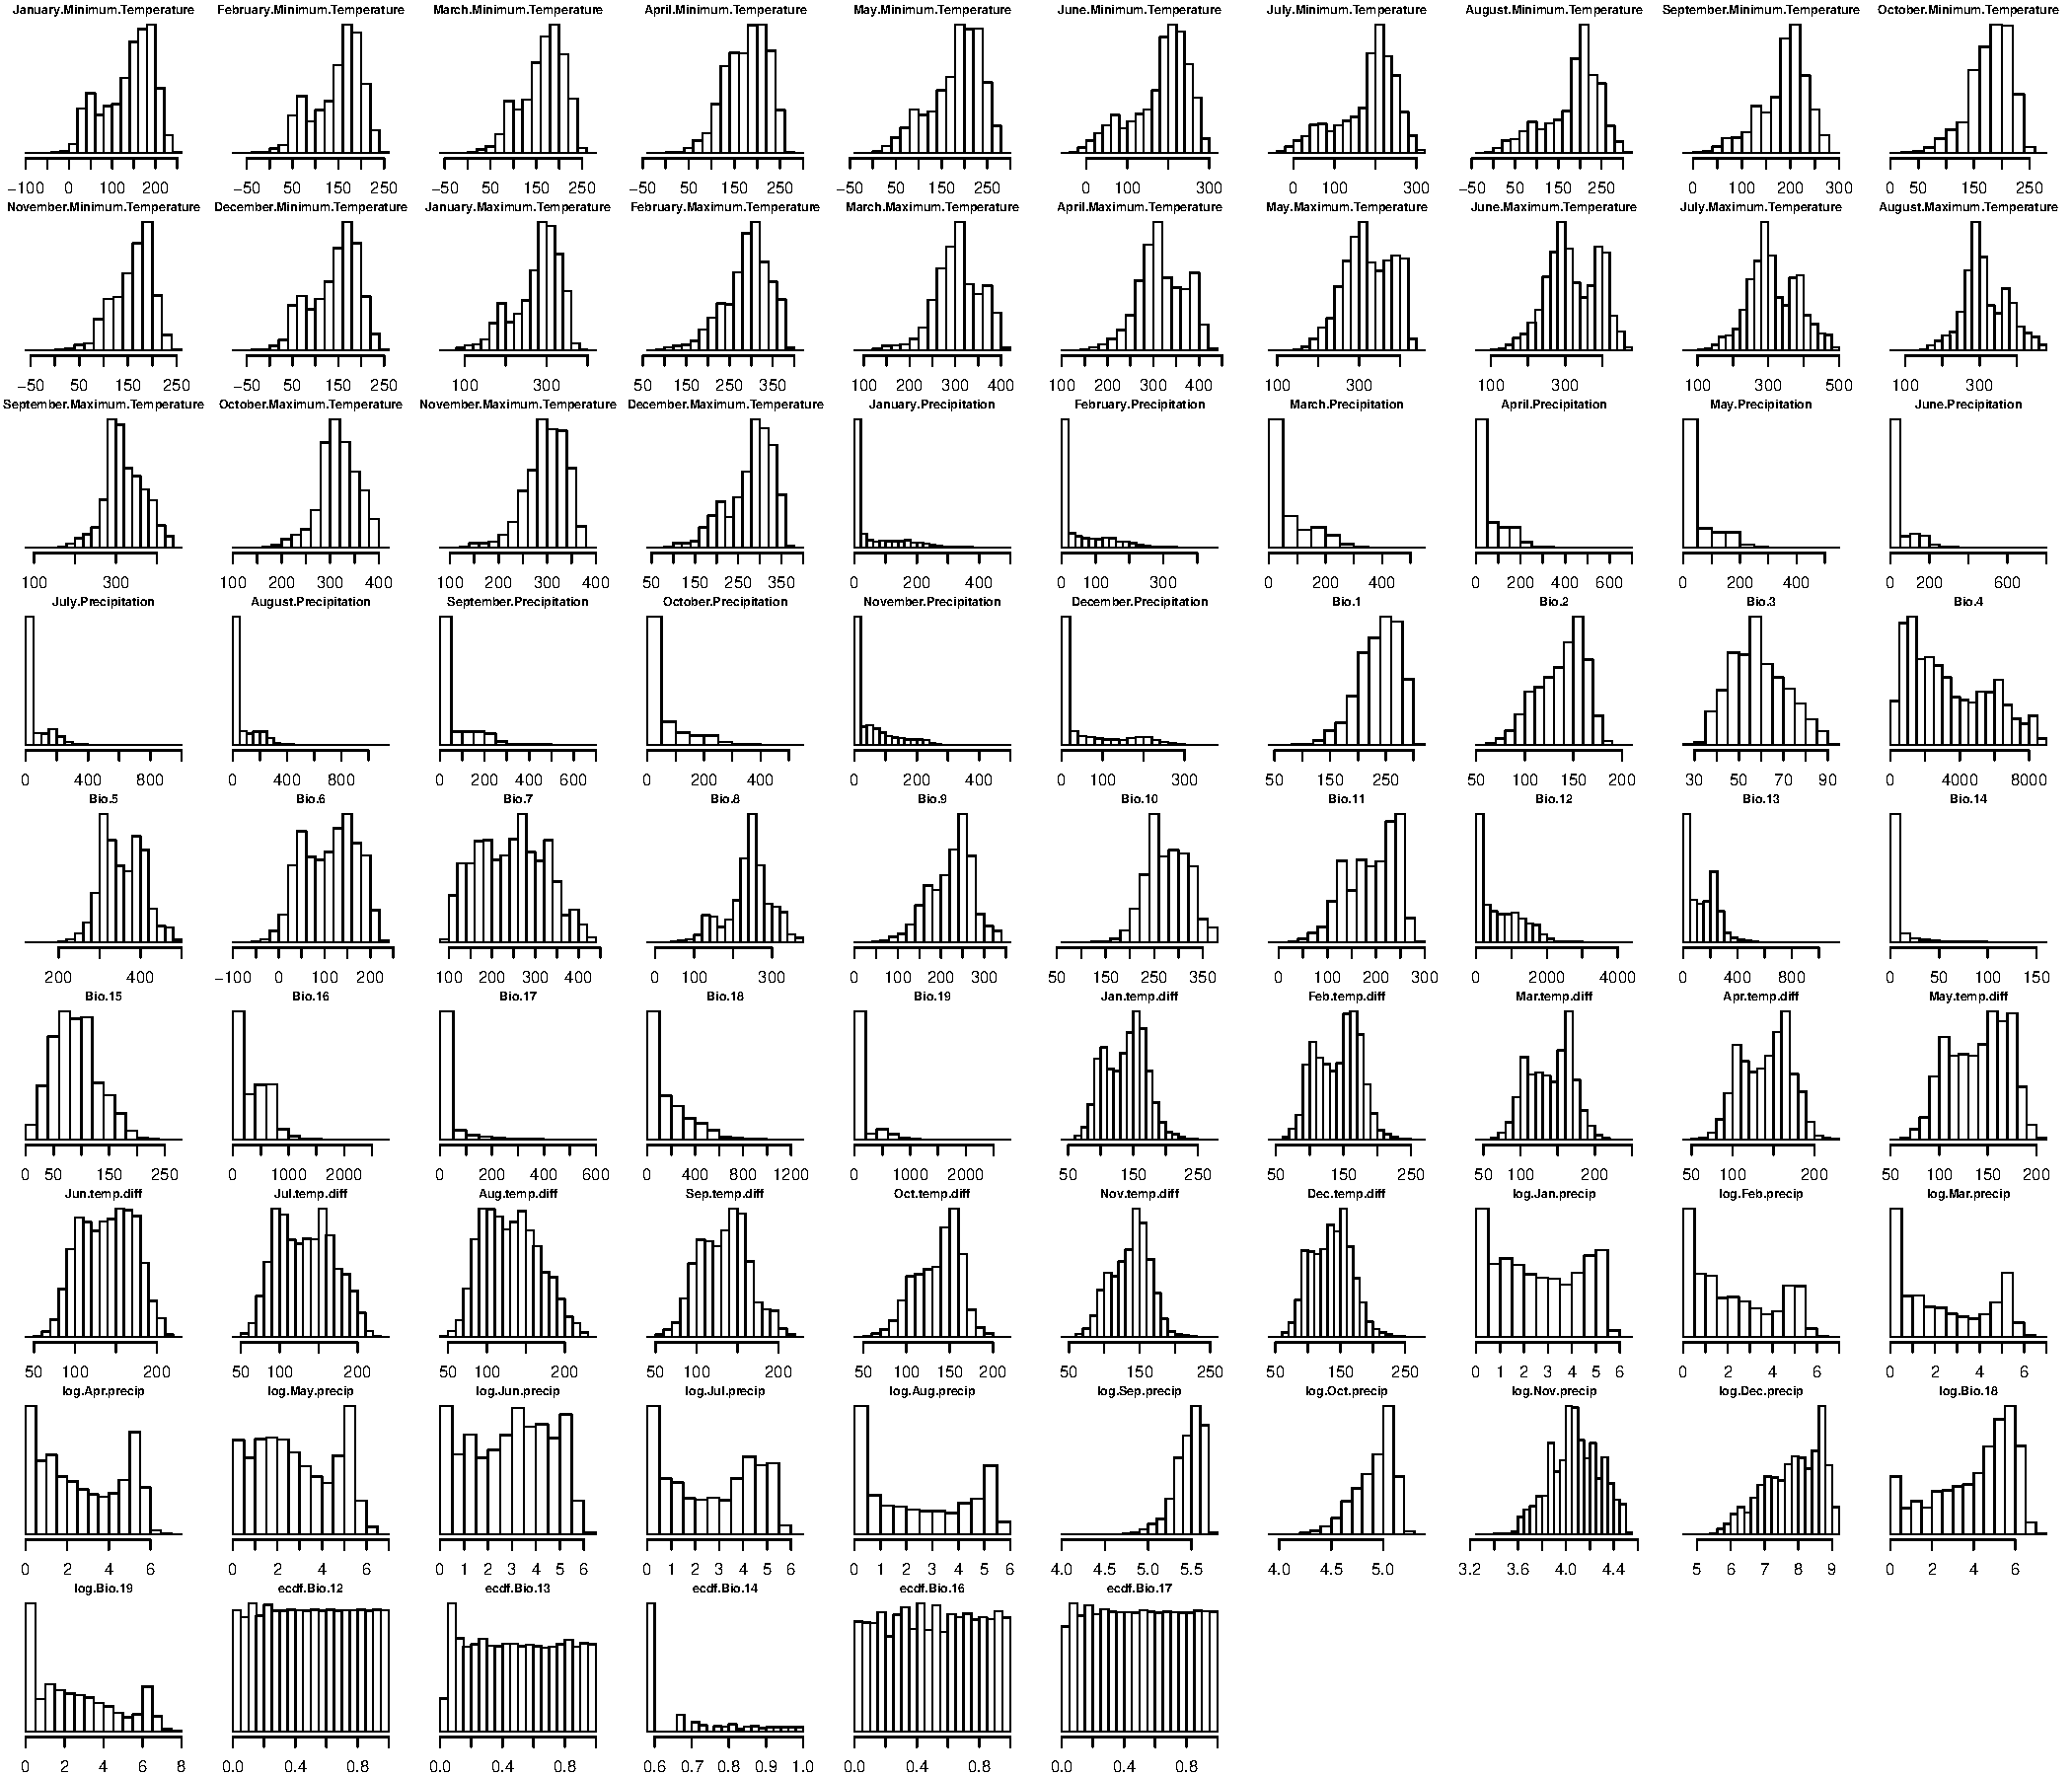
\includegraphics{data-preparation-histograms.pdf}
    \caption{Distributions of $n=86$ environmental features.}  
    \label{fig:histograms}
  \end{center}
\end{figure}

Now we create a new dataset of rescaled environmental data. Data are rescaled by subtracting the raster mean and dividing by the raster standard deviation. Layers in the forecasting datasets are rescaled by the mean and standard deviation of the baseline dataset. Variables which are ecdf transforms are not rescaled.

\begin{Schunk}
\begin{Sinput}
> environmental.data.rs <- raster(environmental.data)   #raster brick to hold rescaled environmental data
> for(i in 1:81) environmental.data.rs <- addLayer(environmental.data.rs,rescale.raster(environmental.data[[i]]))  #rescale variables
> for(i in 82:86) environmental.data.rs <- addLayer(environmental.data.rs,environmental.data[[i]]) #don't rescale variables with ecdf transforms
> names(environmental.data.rs) <- unlist(variable.names)
> #data.a1b.rs <- raster(data.a1b)   #raster brick to hold rescaled environmental data
> #for(i in 1:81) data.a1b.rs <- addLayer(data.a1b.rs,rescale.raster(environmental.data[[i]], data.a1b[[i]]))  #rescale variables
> #for(i in 82:86) data.a1b.rs <- addLayer(data.a1b.rs,data.a1b[[i]]) #don't rescale variables with ecdf transforms
> #names(data.a1b.rs) <- unlist(variable.names)
> 
> #data.a2a.rs <- raster(data.a2a)   #raster brick to hold rescaled environmental data
> #for(i in 1:81) data.a2a.rs <- addLayer(data.a2a.rs,rescale.raster(environmental.data[[i]], data.a2a[[i]]))  #rescale variables
> #for(i in 82:86) data.a2a.rs <- addLayer(data.a2a.rs,data.a2a[[i]]) #don't rescale variables with ecdf transforms
> #names(data.a2a.rs) <- unlist(variable.names)
> 
> #data.b2a.rs <- raster(data.b2a)   #raster brick to hold rescaled environmental data
> #for(i in 1:81) data.b2a.rs <- addLayer(data.b2a.rs,rescale.raster(environmental.data[[i]], data.b2a[[i]]))  #rescale variables
> #for(i in 82:86) data.b2a.rs <- addLayer(data.b2a.rs,data.b2a[[i]]) #don't rescale variables with ecdf transforms
> #names(data.b2a.rs) <- unlist(variable.names)
> 
> save.image('culex-v2.RData')
\end{Sinput}
\end{Schunk}

Here we plot the rescaled data distributions for the baseline data (Fig. \ref{fig:scaled-histograms}).

\begin{Schunk}
\begin{Sinput}
> #plot rescaled data distributions
> #x11()
> par(mar=c(2,1,1,1), mfrow=c(9,10))
> for(i in 1:86){
+   hist(environmental.data.rs[[i]], xlab='', ylab='', axes=FALSE, main=variable.names[i,1], cex.main=0.7)
+   axis(1)
+ }
\end{Sinput}
\end{Schunk}
% 
\begin{figure}
  \begin{center}
    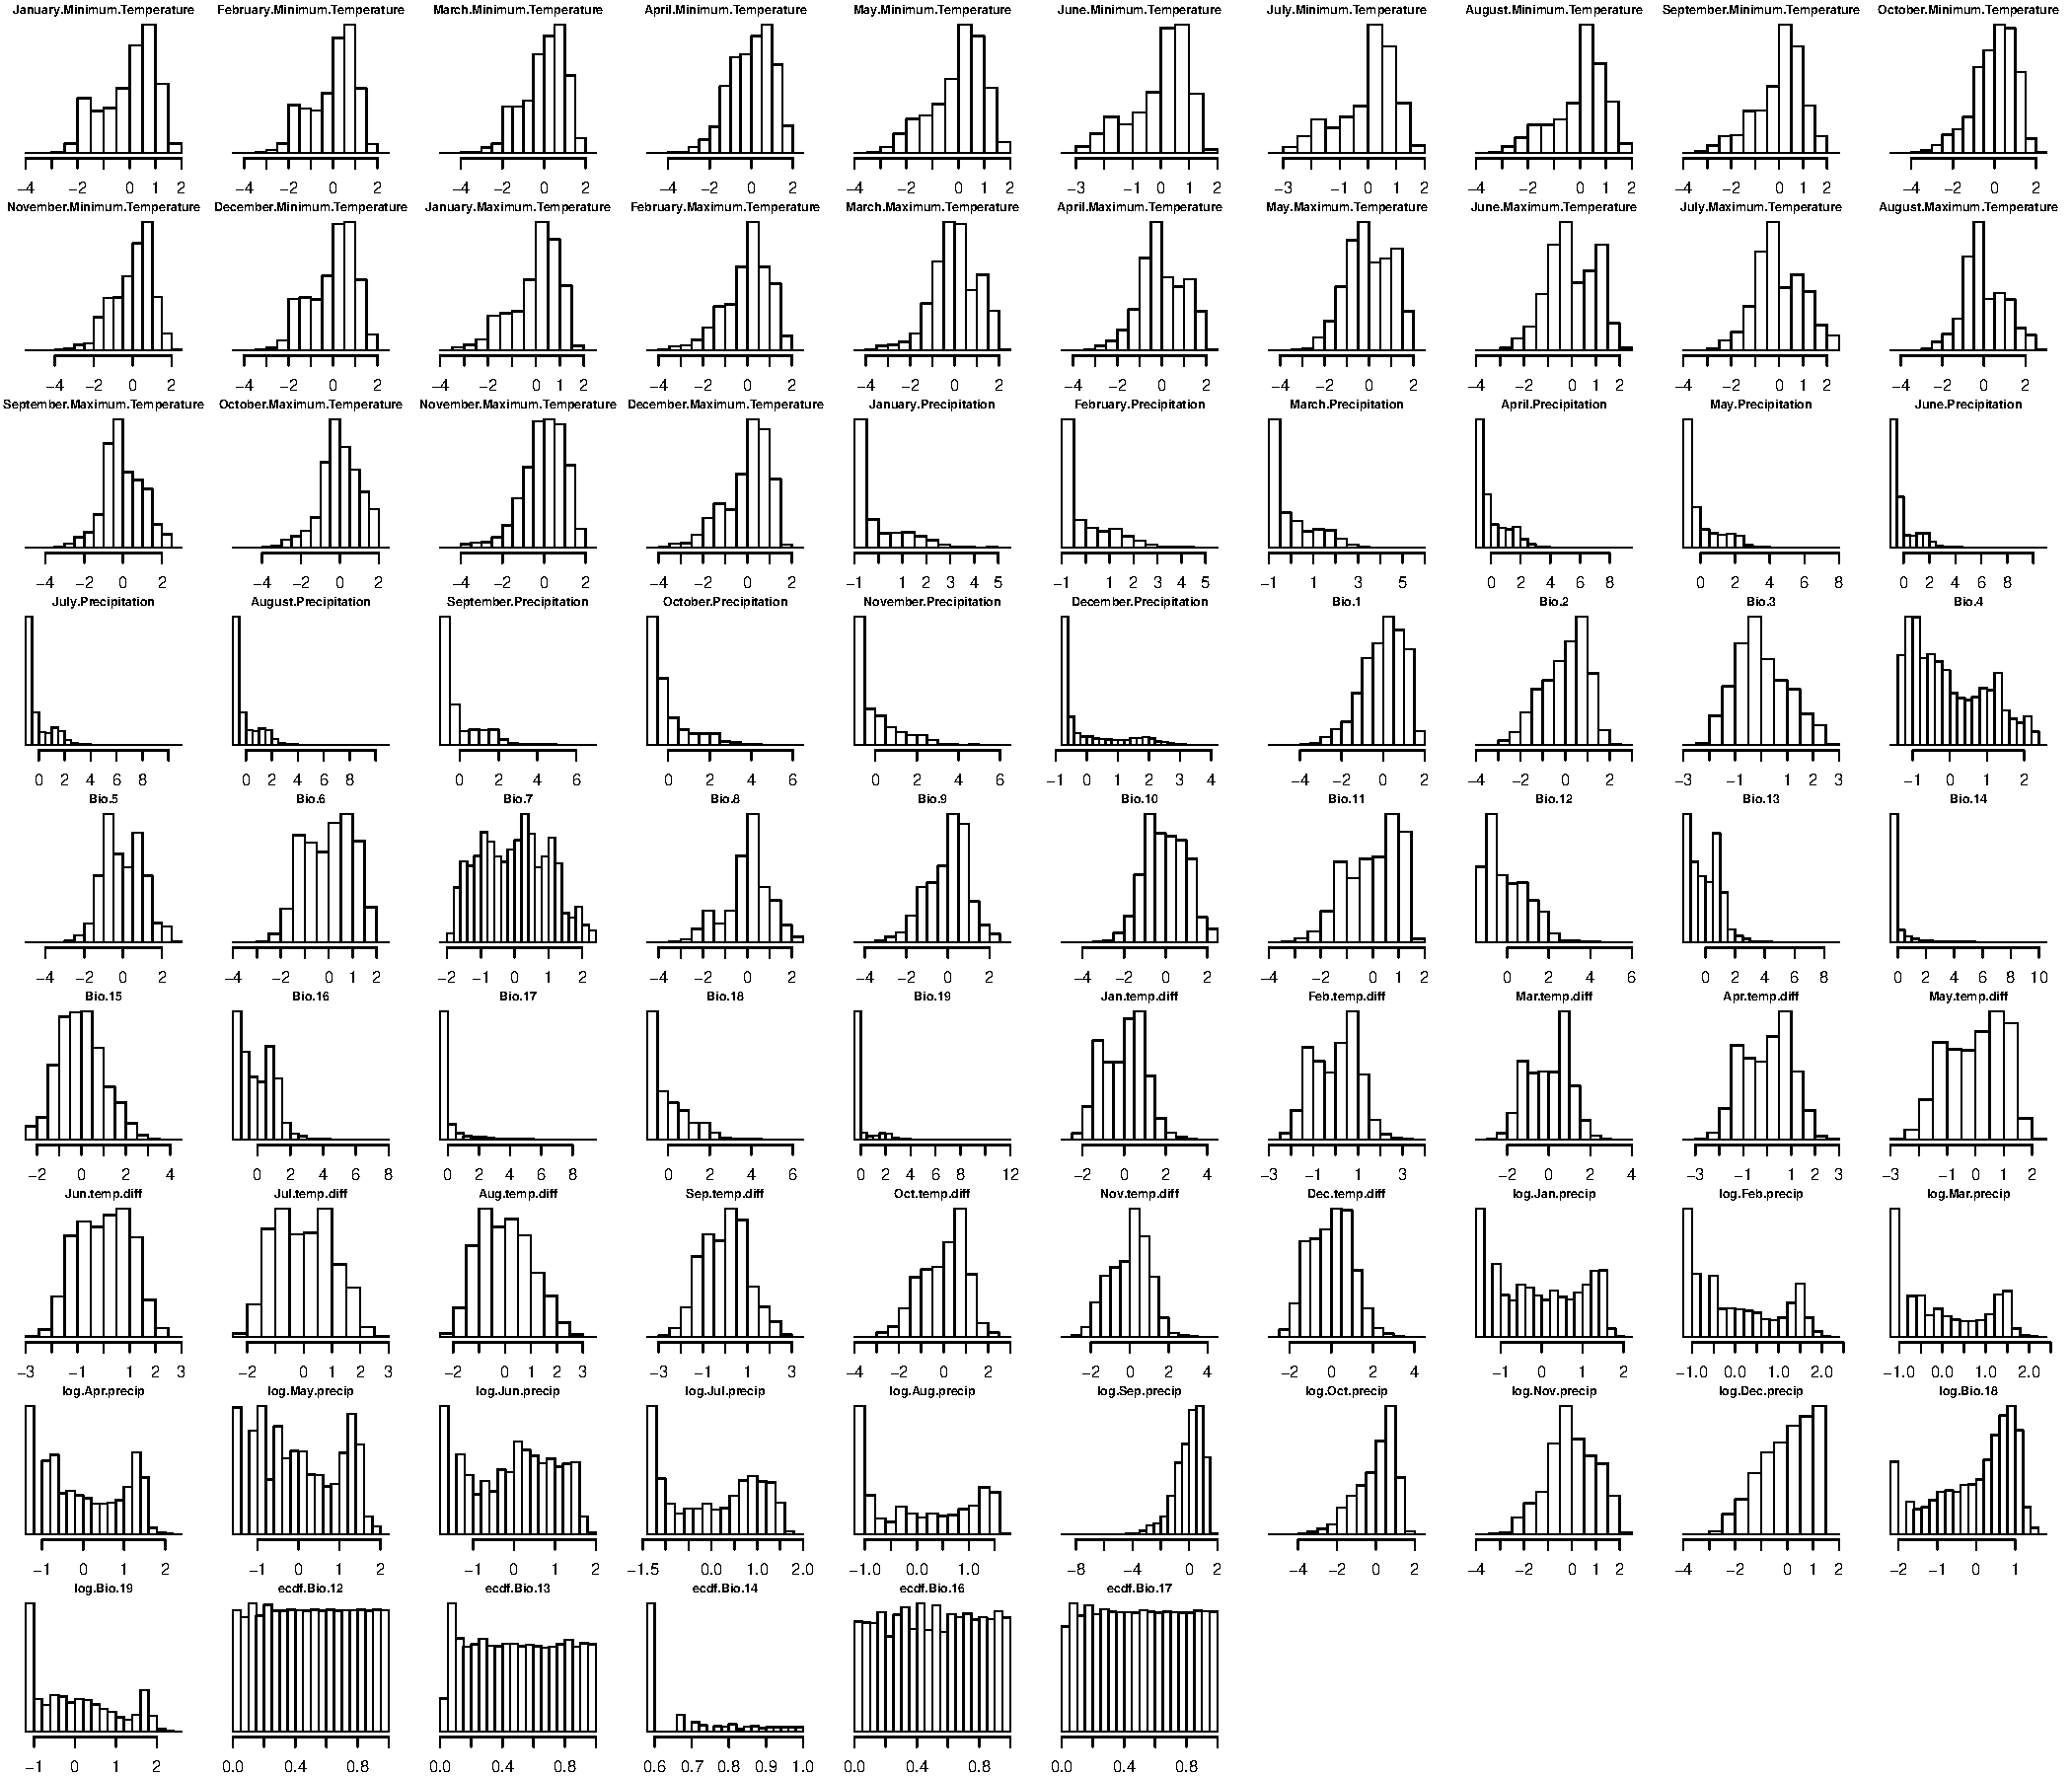
\includegraphics{data-preparation-plotRescale.pdf}
    \caption{Distributions of $n=86$ rescaled environmental features.}  
    \label{fig:scaled-histograms}
  \end{center}
\end{figure}

\begin{Schunk}
\begin{Sinput}
> #plot rescaled data maps
> #x11()
> par(mar=c(0.5,0.5,0.5,0.5), mfrow=c(9,10))
> for(i in 1:86) plot(environmental.data.rs[[i]], main='', cex.main=0.7, axes=FALSE, legend=FALSE)
\end{Sinput}
\end{Schunk}

\begin{figure}
  \begin{center}
    \includegraphics{data-preparation-rescaleMaps.pdf}
    \caption{Maps of $n=86$ rescaled environmental features.}  
    \label{fig:scaled-maps}
  \end{center}
\end{figure}

\section{Principal components analysis}

In the section we perform a principal components analysis of the rescaled baseline environmental data.

\begin{Schunk}
\begin{Sinput}
> set.seed(10281979)
> n <- 5e4
> z <- extract(environmental.data.rs, randomPoints(environmental.data.rs, n))
> pca <- prcomp(z)
\end{Sinput}
\end{Schunk}

\begin{Schunk}
\begin{Sinput}
> par(mfrow=c(2,2))
> plot(pca, main='Scree plot', cex.main=0.5)
> plot(pca$x[,1:2], main='Principal Components Analysis (n=50,000)', pch=19, cex=0.02, col='grey', cex.main=0.5, xlab='PC1', ylab='PC2')
> plot(pca$x[1:2000,1:2], main='Principal Components Analysis (n=2,000)', pch=19, cex=0.02, col='grey', cex.main=0.5, xlab='PC1', ylab='PC2')
> #scatterplot <- scatterplot3d(pca$x[1:3000,1],pca$x[1:3000,2],pca$x[1:3000,3], pch=19, cex.symbols=0.5, type='p', highlight.3d=TRUE, xlab='PC1', ylab='PC2', zlab='PC3', angle=40)
> #scatterplot$points3d(pca$x[1:3000,1],pca$x[1:3000,2],rep(-10,3000), pch=19, cex=0.5, col='grey')
\end{Sinput}
\end{Schunk}

\begin{figure}
  \begin{center}
    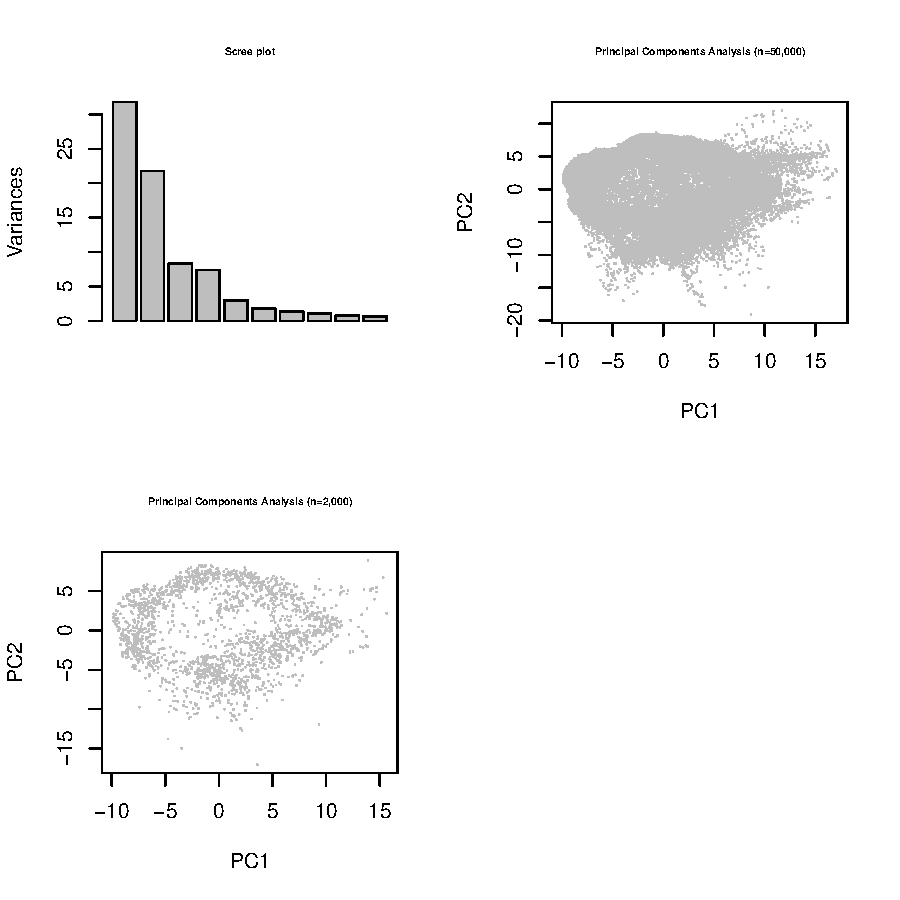
\includegraphics{data-preparation-plotPCA.pdf}
    \caption{Principal components analysis of $n=86$ environmental features.}  
    \label{fig:pca4}
  \end{center}
\end{figure}

Approximately 55\% of the variation in environmental covariates is contained in just the first two principal components (Fig. \ref{fig:pca}). Curiously, the first two principal components are distributed in a kind of ring. This is more obvious in the plot of 2,000 points than the plot of ~50,000 points, which is just too dense.

\section{Point data}

In this section we prepare point data. First, we load the coordinates of collection sites. The raw data may be downloaded from \url{http://www.mosquitomap.prg/}.

\begin{Schunk}
\begin{Sinput}
> #load Cx. pipiens data
> pipiens <- read.csv('pipiens.csv', skip=2)
> pipiens.coords <- cbind(pipiens$DecimalLongitude, pipiens$DecimalLatitude)
> quinq <- read.csv('quinq.csv', skip=2)
> quinq.coords <- cbind(quinq$DecimalLongitude, quinq$DecimalLatitude)
> salinarius <- read.csv('salinarius.csv', skip=2)
> salinarius.coords <- cbind(salinarius$DecimalLongitude, salinarius$DecimalLatitude)
\end{Sinput}
\end{Schunk}

\subsection{Occurrence points}

\begin{Schunk}
\begin{Sinput}
> plot(pipiens.coords, pch=20, cex=0.6)
> #plot(wrld_simpl[wrld_simpl$REGION==2,], add=TRUE)  # plot just Africa
> plot(wrld_simpl, add=TRUE, border='grey')
\end{Sinput}
\end{Schunk}

\begin{figure}
  \begin{center}
    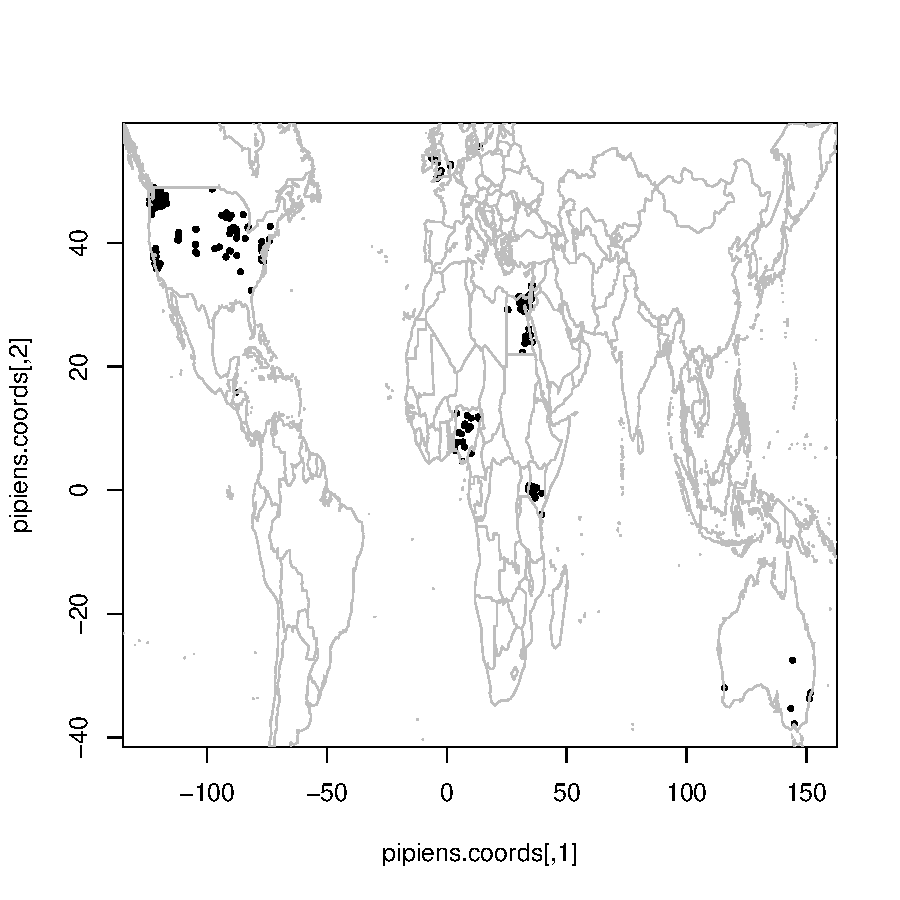
\includegraphics{data-preparation-occurrence.pdf}
    \caption{Distribution of sampling points for \textit{Culex pipiens}.}  
    \label{fig:Cx-pipiens}
  \end{center}
\end{figure}

\subsection{Data extraction and background points}

Now we extract the environmental variables at the presence locations.

\begin{Schunk}
\begin{Sinput}
> pipiens.presence <- data.frame(extract(environmental.data.rs, pipiens.coords))
\end{Sinput}
\end{Schunk}

Some points are NA. (Paricularly those outside Africa.) We drop these.

\begin{Schunk}
\begin{Sinput}
> z <- which(is.na(pipiens.presence[,1]))
> plot(environmental.data.rs[[1]])
> points(pipiens.coords, pch=21, bg='yellow', cex=0.6)
> pipiens.presence <- pipiens.presence[-z,]
> n.presence <- dim(pipiens.presence)[1]
> pts.presence <- pipiens.coords[-z,]
\end{Sinput}
\end{Schunk}

We can now determine that there are a total of $n_p=2469$ presence records. For later testing, we randomly select $n_p$ environmental data points from the background distribution (Fig. \ref{fig:presence-background}).

\begin{Schunk}
\begin{Sinput}
> #simulate background data
> set.seed(10281979)
> backgr.pts <- randomPoints(environmental.data.rs, n.presence)
> data.background <- data.frame(extract(environmental.data.rs, backgr.pts))
> cols <- colorRampPalette(c('darkorange4', 'khaki1'), interpolate='linear')
> plot(environmental.data[[37]]/10, col=(cols(100)), main='Presence/background points')
> points(pipiens.coords, pch=21, bg='yellow', cex=0.6)
> points(backgr.pts, pch=21, bg='grey', cex=0.6)
> plot(wrld_simpl[wrld_simpl$REGION==2,], add=TRUE)
> legend('topright', pch=21, pt.bg=c('yellow','grey'), legend=c('Cx. pipiens', 'Background'), bty='n', cex=0.7)
> text(-17,-25,'Annual mean', pos=4, cex=0.8)
> text(-17,-28, 'temperature (degrees C)', pos=4, cex=0.8)
> save.image('culex-v3.RData')
\end{Sinput}
\end{Schunk}

\begin{figure}
  \begin{center}
    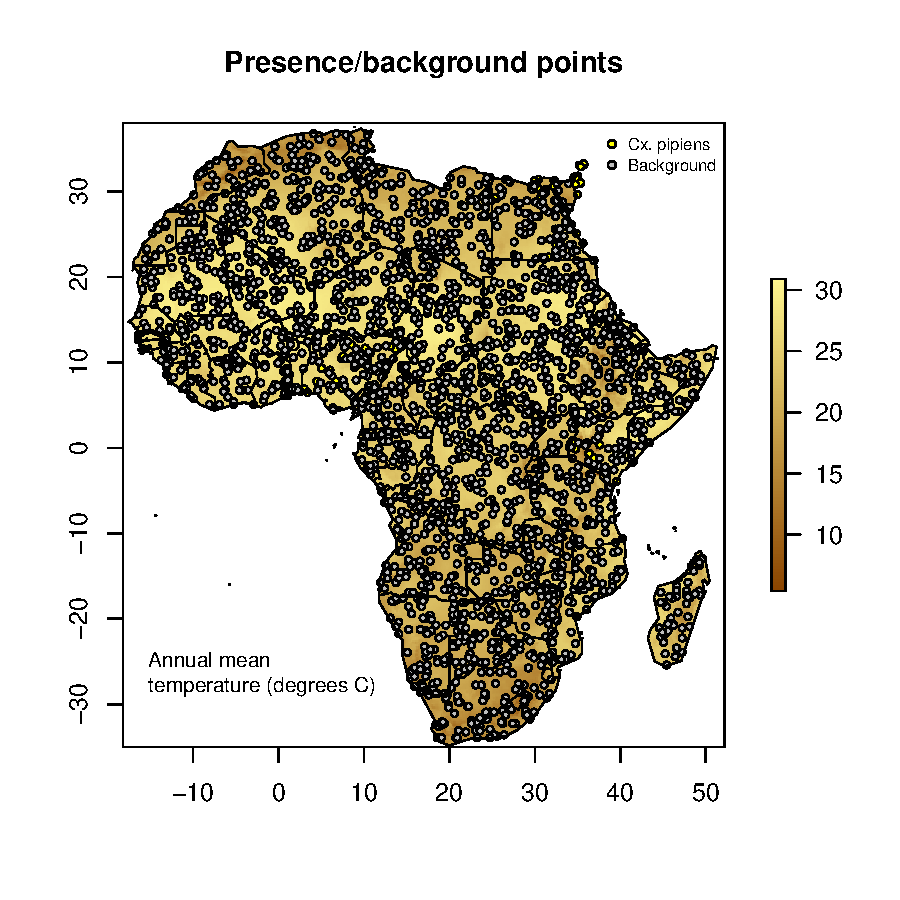
\includegraphics{data-preparation-background.pdf}
    \caption{Distribution of sampling points for all \emph{Cx. pipiens} and a balanced random sample of background points.}  
    \label{fig:presence-background}
  \end{center}
\end{figure}

\subsection{Data splitting}

To enable quantifying model performance later on an independent set of data, the presence points are randomly split into training (80\%) and testing (20\%) sets, yielding a total of $\tilde n_p = 1976$ observations in the training sets for presence and background points.


\begin{Schunk}
\begin{Sinput}
> #Split train and test datasets
> set.seed(10281979)
> train.presence.id <- sample(seq(1,n.presence),ceiling(0.8*n.presence))
> train.background.id <- sample(seq(1,n.presence),ceiling(0.8*n.presence))
> train.presence <- pipiens.presence[c(train.presence.id),]
> train.background <- data.background[c(train.background.id),]
> test.presence <- pipiens.presence[-c(train.presence.id),]
> test.background <- data.background[-c(train.presence.id),]
\end{Sinput}
\end{Schunk}

\section{Visualization in principal components}

Here we visualize the \emph{Cx. pipiens} training data in the space of the first two principal components (Fig. \ref{fig:pca}).

\begin{Schunk}
\begin{Sinput}
> data.presence.pca <- predict(pca, train.presence)
> save.image('culex-v4.RData')
\end{Sinput}
\end{Schunk}

\begin{Schunk}
\begin{Sinput}
> #pdf(file='data-preparation-pca.pdf',w=6.5, h=5)
> par(mfrow=c(1,2))
> plot(pca, main='A. Scree plot', cex.main=0.8)
> plot(pca$x[1:2000,1:2], main='B. Principal Components Analysis', pch=19, cex=0.02, col='grey', cex.main=0.8)
> points(data.presence.pca[,1:2], pch=21, bg='yellow', cex=0.3)
> legend('topright', pch=21, pt.bg=c('yellow'), legend=c('Cx. pipiens present'), bty='n', cex=0.7)
> convex.hull <- chull(data.presence.pca[,1:3])
> lines(data.presence.pca[c(convex.hull, convex.hull[1]),1:2 ], lwd=1.5)
> #dev.off()
\end{Sinput}
\end{Schunk}

\begin{figure}
  \begin{center}
    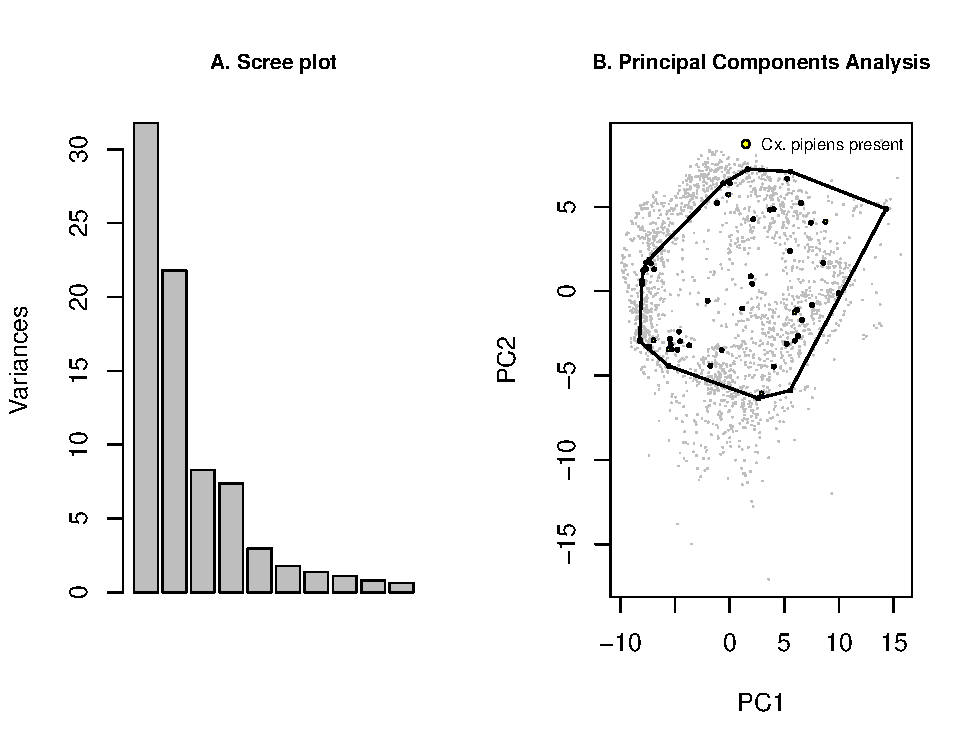
\includegraphics{data-preparation-pca.pdf}
    \caption{Sampling points where \emph{Cx. pipiens} is present vs. absent in the space of the first two principal components of the environmental features. Evidently, \emph{Cx. pipiens} is environmentally widely dispersed. Equivalently, we would say that it has a large niche.}  
    \label{fig:pca}
  \end{center}
\end{figure}

Evidently, despite the relatively restricted geographic range in Africa, the range of environmental conditions where \emph{Cx. pipiens} has been collected covers a large fraction (more than half) of the range of conditions actually realized in nature. This suggests that model fitting and estimation of performance with respect to the absence records would be inappropriate.

Here we plot again the training and background points.

\begin{Schunk}
\begin{Sinput}
> #simulate background data
> set.seed(10281979)
> #backgr.pts <- randomPoints(environmental.data.rs, n.presence)
> #data.background <- data.frame(extract(environmental.data.rs, backgr.pts))
> #cols <- colorRampPalette(c('darkorange4', 'khaki1'), interpolate='linear')
> plot(environmental.data[[37]]/10, col=(cols(100)), main='Presence/background points')
> points(pts.presence, pch=21, bg='yellow', cex=0.6)
> points(backgr.pts, pch=21, bg='grey', cex=0.6)
> plot(wrld_simpl[wrld_simpl$REGION==2,], add=TRUE)
> legend('topright', pch=21, pt.bg=c('yellow','grey'), legend=c('Cx. pipiens', 'Background'), bty='n', cex=0.7)
> text(-17,-25,'Annual mean', pos=4, cex=0.8)
> text(-17,-28, 'temperature (degrees C)', pos=4, cex=0.8)
\end{Sinput}
\end{Schunk}

\end{document}
